\documentclass[a4paper, 12pt, titlepage]{report}

%Taal: Nederlands ("Inhoudsopgave", "Hoofdstuk",...)
\usepackage{graphicx}
\usepackage{subcaption}
\usepackage{algorithmic}
\usepackage{amsmath, amssymb, textcomp, mathtools}

%Hyperlinks
\usepackage{hyperref}

%Opmaak hyperlinks
\hypersetup{colorlinks=false,	urlcolor=cyan,pdfborder=0 0 0}

%Geen nummering bij secties en hoofdstukkden
\setcounter{secnumdepth}{-1} 

%geen indents
\setlength\parindent{0pt}

\usepackage{listings}
\lstset{
language=Matlab, % choose the language of the code
%basicstyle=10pt, % the size of the fonts that are used for the code
numbers=left, % where to put the line-numbers
numberstyle=\footnotesize, % the size of the fonts that are used for the line-numbers
stepnumber=1, % the step between two line-numbers. If it's 1 each line will be numbered
numbersep=5pt, % how far the line-numbers are from the code
%backgroundcolor=\color{grey}, % choose the background color. You must add \usepackage{color}
showspaces=false, % show spaces adding particular underscores
showstringspaces=false, % underline spaces within strings
showtabs=false, % show tabs within strings adding particular underscores
frame=single, % adds a frame around the code
%tabsize=2, % sets default tabsize to 2 spaces
%captionpos=b, % sets the caption-position to bottom
breaklines=true, % sets automatic line breaking
breakatwhitespace=false, % sets if automatic breaks should only happen at whitespace
escapeinside={\%*}{*)} % if you want to add a comment within your code
}


%"Figuur" in vet
\makeatletter
\renewcommand{\fnum@figure}{\small\textbf{\figurename~\thefigure}}
\makeatother

\usepackage[dutch]{babel}
\begin{document}

\title{\textbf{Numerieke Modellering en Benadering}\\\textit{Practicum 1: Eigenwaardenproblemen}\\}
\author{De Wolf Peter\\ Vekemans Wout}

\date{\today}
\begin{titlepage}
	\maketitle
	\thispagestyle{empty}
\end{titlepage}

\newpage
\tableofcontents

\listoffigures

\newpage

\section{Inleiding}
In dit practicum onderzoeken we methoden voor het bepalen van eigenwaarden van volle matrices. In een eerste sectie beschouwen we enkele theoretische eigenschappen van de methoden. In een tweede sectie worden de convergentie-eigenschappen van de methoden onderzocht aan de hand van MATLAB-experimenten. In de derde en laatste sectie gaan we dieper in op \'e\'en van de methoden, namelijk de Jacobi-methode.
\section{Theoretische eigenschappen}


\subsection{Opgave 1}
Gelijktijdige iteratie is een andere naam voor het toepassen van de methode van de machten op meerdere kolommen van $A$ tegelijk. Zo kunnen de grootste $n$ eigenwaarden van de matrix $A$ gevonden worden.  Om met gelijktijdige iteratie de kleinste $n$ eigenwaarden van A te berekenen is het voldoende om het algoritme toe te passen op $A^{-1}$ in plaats van op $A$. Dit is makkelijk in te zien. De eigenwaarden van de inverse van een singuliere matrix $A$ zijn gelijk aan het omgekeerde van de eigenwaarden van $A$.\\
\begin{subequations} \label{eq:simIt}
\begin{align}
 Ax  = \lambda x \\
A\frac{1}{\lambda}x =  x\\
A^{-1}A\frac{1}{\lambda}x  =  A^{-1}x\\
A^{-1}x  =  \frac{1}{\lambda}x
\end{align}
\end{subequations}

Als we dit algoritme uitschrijven krijgen we volgende pseudocode:\\
\begin{algorithmic}
 \STATE Initialiseer $\hat{Q}^{(0)} \in \mathbb{R}^{m \times n}$ met $n$ orthonormale kolommen.
\FOR	 {$k = 1,2,...$}
\STATE $Z = A^{-1}\hat{Q}^{k-1}$
\STATE $\hat{Q}^{k}\hat{R}^{k} = Z$
\ENDFOR
\end{algorithmic}
Dit zal convergeren naar de $n$ grootste eigenwaarden van $A^{-1}$, die zoals eerder aangetoond in \eqref{eq:simIt} overeenkomen met de $n$ kleinste eigenwaarden van $A$.

\subsection{Opgave 2}
\paragraph{a)} 
De Rayleigh quoti\"ent iteratie convergeert zeer snel naar de juiste waarde van de eigenwaarden van $A$. Elke iteratiestap verdrievoudigt het aantal juiste cijfers. Elke stap dient er wel een stelsel te worden opgelost dat meer en meer singulier wordt naarmate de benadering voor de eigenwaarde juister wordt. Het betreft het stelsel
\begin{equation}\label{eq:rayleighstelsel}
 (A=\lambda^{(k-1)}I)w = v^{(k-1)}
\end{equation}
Als $\lambda$ dichter en dichter bij een eigenwaarde van $A$ komt wordt $A-\lambda^{(k-1)}I$ meer en meer singulier, en zal de inverse van deze matrix, die nodig is om \eqref{eq:rayleighstelsel} op te lossen, ervoor zorgen dat de vector $w$ enorm wordt opgeblazen. De vector zal echter wel in de juiste richting blijven wijzen en wordt genormeerd, waardoor dit geen problemen oplevert.\\
\paragraph{b)}
Gegeven een matrix $A \in \mathbb{R}^{m \times m}$ en een vector $x \in \mathbb{R}^{m \times 1}$, waarbij $x$ een benadering is voor een eigenvector van $A$. Toon aan dat de oplossing $\rho \in \mathbb{R}$ van het minimalisatieprobleem 
\begin{equation}
 \underset{\rho \in \mathbb{R}}{\text{min}}|| Ax-\rho x||_{2}
\end{equation}
overeenkomt met het Rayleighquoti\"ent van $x$.\\
Dit probleem lijkt op het standaard kleinste kwadraten probleem $Ax \approx b$. We proberen nu een $\rho$ te vinden zodat $||Ax-\rho x||_{2}$ geminimaliseerd wordt. De overeenkomstige normaalvergelijkingen (cf $A^TAx = A^Tb)$ worden gegeven door 
\begin{subequations}
\begin{align}
  x^Tx\rho = x^TAx\\
 \rho = \frac{x^TAx}{x^Tx}=r(x)
\end{align}
\end{subequations}
waarbij $r(x)$ het Rayleigh quoti\"ent van $x$ voorstelt.

\subsection{Opgave 3}
\paragraph{a)}
Gegeven een schatting voor de eigenvector horend bij de derde kleinste eigenwaarde van een symmetrische matrix $A \in \mathbb{R}^{m \times m}$ , bepaal de bijhorende eigenwaarde.\\
Als een benadering $v$ voor een eigenvector gekend is, kan er m.b.v. het Rayleigh quoti\"ent $\mu$ van die vector een benadering van de bijhorende eigenwaarde worden berekend.
\begin{equation}
	\mu = \frac{v^TAv}{v^Tv}
	\label{eqn:rayleighquotient}
\end{equation}
Daarna kan er met een inverse iteratiestap een betere benadering voor de eigenvector worden berekend. Als deze stappen $k$ keer herhaald worden spreekt men van Rayleigh quoti\"ent iteratie. Deze methode kent een kubische convergentie voor een symmetrische matrix. \\
Om het algoritme effici\"ent te kunnen uitvoeren moet de matrix eerst gereduceerd worden tot Hessenberg vorm, dit vraagt $\mathcal{O}(\frac{10}{3}m^3)$ flops. Na deze reductie heeft Rayleigh quoti\"ent iteratie maar $\mathcal{O}(m)$ flops per iteratiestap nodig, in tegenstelling tot de $\mathcal{O}(m^3)$ flops per stap indien er niet gereduceerd wordt. 
\paragraph{b)}
Gegeven een symmetrische matrix $A \in \mathbb{R}^{m \times m}$, bepaal de eigenwaarde het dichts gelegen bij een getal $\alpha$.\\
Om een schatting van een eigenvector te krijgen, maken we gebruik van 1 iteratiestap van inverse iteratie. Hiervoor lossen we het stelsel \eqref{eq:rayleighstelsel} op, met $\alpha$ als waarde voor $\lambda$, en $v$ een willekeurige vector met $||v||_2 = 1$.\\ 
De vector $w$ die we dan krijgen kunnen we gebruiken als startvector voor Rayleigh quoti\"ent iteratie. Dit heeft kubische convergentie en is dus het snelst van alle beschouwde algoritmes. Zoals hierboven vermeld is er eerst reductie tot Hessenberg vorm nodig om het aantal flops per iteratiestap te verminderen. 
\section{Convergentie-experimenten}
Voor al deze experimenten wordt gebruik gemaakt van een volle, re\"ele symmetrische matrix A. We laden hiervoor de gegeven matrix $mat1.txt$ in in MATLAB.

\subsection{Opgave 4}
Het uitvoeren van het $spy$-commando laat zien dat er geen enkel $non-zero$ element in de matrix zit. De uitvoering van het QR-algoritme op een matrix met die afmetingen (nog steeds relatief klein) zou zeer veel werk vragen. \\
Na het reduceren tot Hessenberg vorm zien we dat alle elementen onder de eerste benedendiagonaal nul zijn geworden. Verdere analyse leert ons dat ook de elementen boven de eerste bovendiagonaal allemaal van grootteorde $\epsilon_{mach}$ zijn. Als we de Hessenberg vorm van de matrix afronden tot op 15 decimalen verkijgen we een tridiagonale matrix.(zie figuur \ref{hessenberg}) Dit komt doordat de originele matrix symmetrisch was. De reductie naar Hessenberg vorm zorgt ervoor dat het algoritme niet op een volledige matrix moet inwerken. Het uitvoeren van het QR-algoritme vraagt nu slechts $\mathcal{O}(n^2)$ flops. 
\begin{figure}[!h]
\begin{subfigure}{.5\textwidth}
\centering
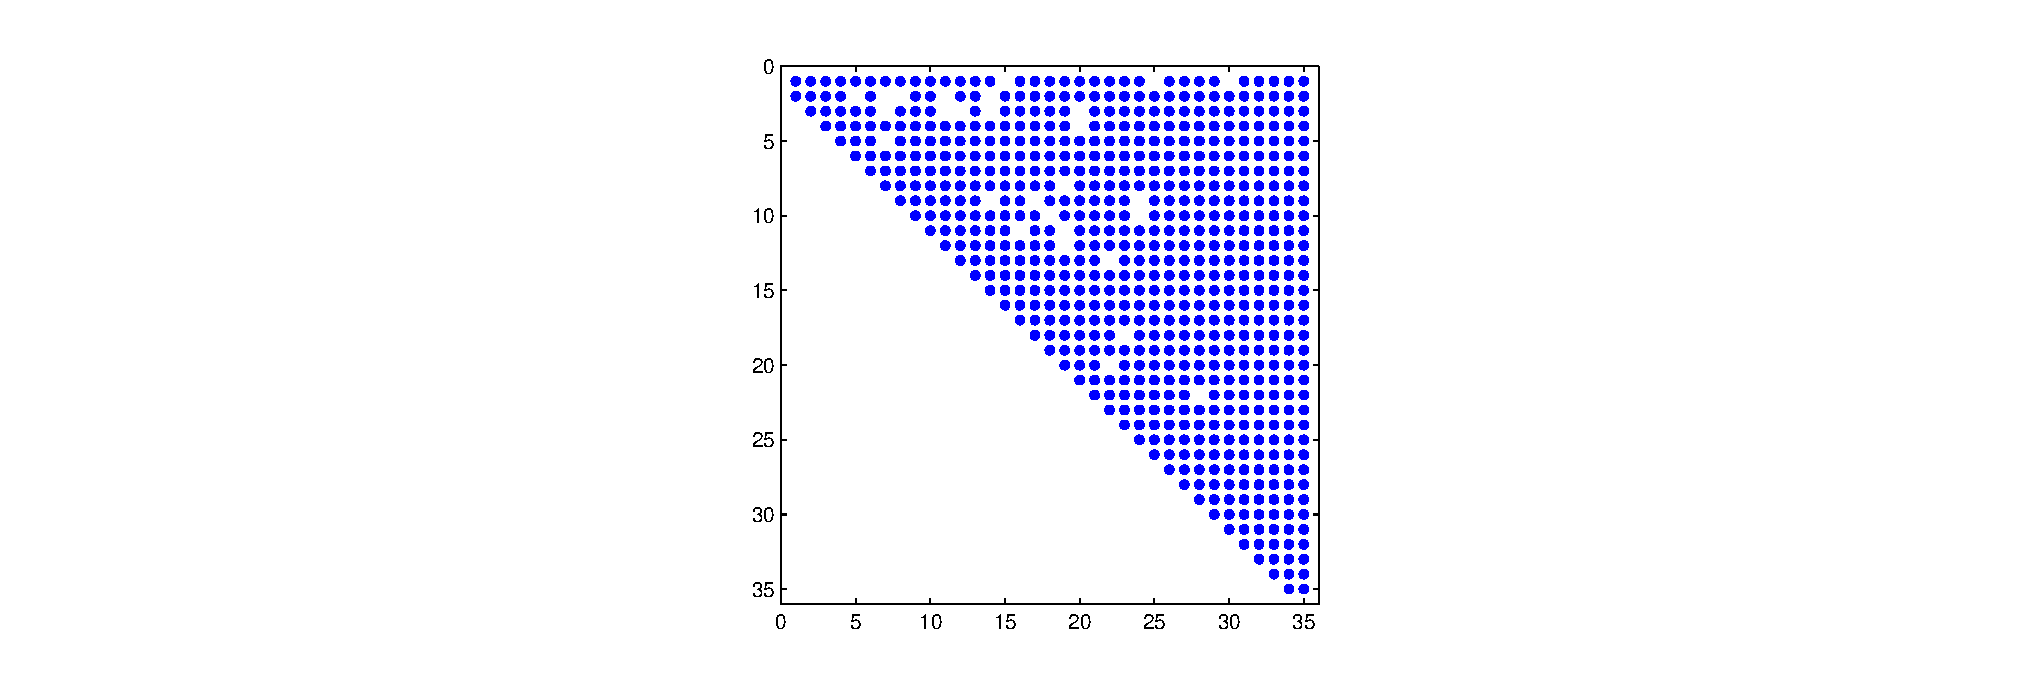
\includegraphics[width=\textwidth]{structuur_hessenberg.eps}
\subcaption{zonder afronden}
\end{subfigure}
\begin{subfigure}{.5\textwidth}
\centering
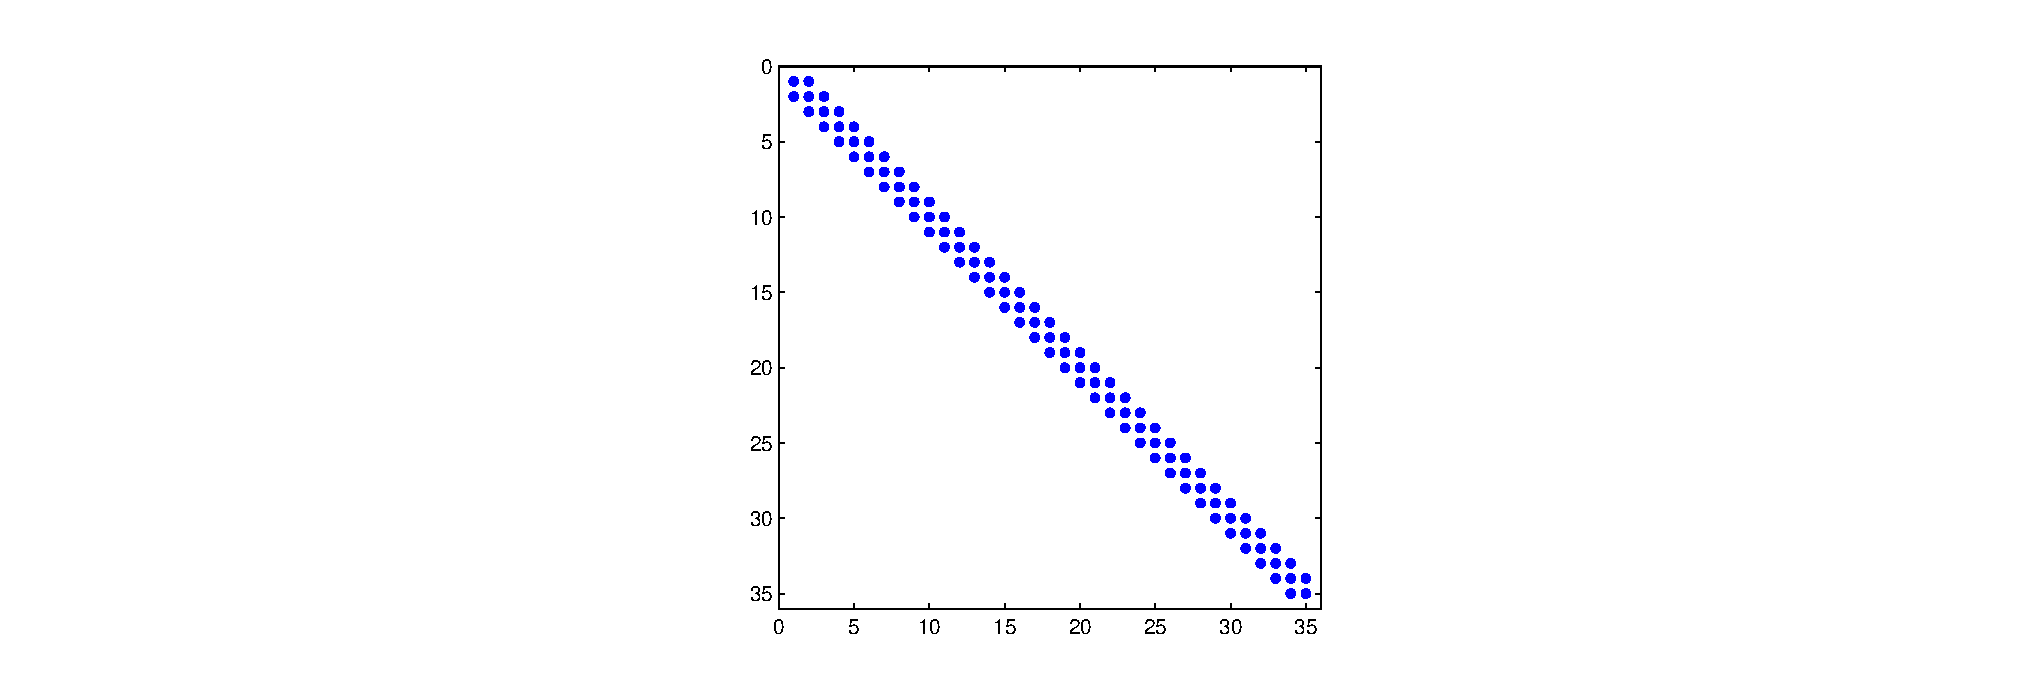
\includegraphics[width=\textwidth]{afgerond.eps}
\subcaption{met afronden}
\end{subfigure}

\caption{Structuur van de Hessenberg matrix}
\label{hessenberg}
\end{figure}

\subsection{Opgave 5}
Het toepassen van de drie verschillende versies van het QR algoritme geeft ons figuur \ref{3QRs}. Het is duidelijjk dat er twee kubisch convergerende methodes zijn, en 1 lineaire. \\
Als maat voor de convergentie gebruiken we de waarde van een element net onder de diagonaal $A$. Dit doen we omdat de matrix convergeert naar een diagonaalmatrix. Hoe dichter de waarde van dat element bij nul ligt, hoe dichter de matrix een diagonaalmatrix benadert. We zien op de grafiek duidelijk dat het residu bij het algoritme zonder shifts lineair convergeert naar 0. De algoritmes met shifts (Rayleigh en Wilkinson) convergeren kubisch en zijn dus veel sneller dan het algoritme zonder shifts. Het is zelfs zo dat de methoden met shift al een absolute fout kleiner dan $10^{-16}$ hebben na een tweetal stappen.\\

\begin{figure}[htb]
	\centering
	\includegraphics[width=\textwidth]{3QRS.eps}
	\caption{Convergentie van verschillende QR algoritmes}
	\label{3QRs}
\end{figure}


Voor het algoritme zonder shifts stemt dit volledig overeen met de theorie. Theorema 28.4 (p. 218 in het handboek) geeft duidelijk aan dat bij het gebruik van QR zonder shifts $A^{(k)}$ lineair convergeert naar een diagonaalmatrix met de eigenwaarden van $A$ als elementen. Deze lineaire convergentie kan sterk verbeterd worden door het gebruik van shifts. \\
Als we bijvoorbeeld het Rayleigh quoti\"ent gebruiken als shift in elke iteratiestap krijgen we kubische convergentie naar de eigenwaarde die hoort bij de eigenvector die benaderd wordt door de laatste kolom van $A$. Dan zijn de berekenden benaderingen $\mu$ en $q_m$ in elke stap gelijk aan diegenen die berekend worden door de Rayleigh quoti\"ent iteratie die gestart wordt met de $m^{de}$ eenheidsvector. Door dit verband is het duidelijk dat het QR algoritme met Rayleigh shift in het beste geval kubisch convergeert. De Rayleigh iteratie doet dit immers ook. Dit is duidelijk te zien op de figuur. \\
Om een resultaat te vinden dat minder afhankelijk is van beginvoorwaarden kunnen we ook Wilkinson shift gebruiken. Hiervoor nemen we een submatrix $B$ uit $A$ en gebruiken we de eigenwaarde van B die het dichtste bij $a_m$ ligt als shift. Dit algoritme garandeert zelfs in het slechtste geval nog kwadratische convergentie, in tegenstelling tot het algoritme met Rayleigh shifts, dat soms helemaal niet convergeert.
\begin{equation}
 B=\begin{bmatrix} a_{m-1} & b_{m-1} \\ b_{m-1} & a_m\end{bmatrix}
\end{equation}


\begin{table}[h]
\begin{center}
\begin{tabular}{r||c|c|c}

Iteratie	&	\textbf{unshifted}	&	\textbf{Wilkinson}	&	\textbf{Rayleigh}	\\
\hline
1	&	7.6359E-01	&	1.8360E-02	&	1.8347E-02	\\
2	&	2.1011E-01	&	9.8332E-07	&	1.2342E-05	\\
3	&	8.0838E-02	&	1.1383E-18	&	9.5580E-15	\\
4	&	3.3388E-02	&	0		&		0	\\
5	&	1.4090E-02	&	0		&		0	\\

\end{tabular}
\caption{Residu van de 3 verschillende methoden, voor de eerste vijf stappen}
\label{errorQR}

\end{center}
\end{table}


\subsection{Opgave 6}
De Rayleigh quoti\"ent iteratie en de Rayleigh shift methode zouden allebei kubisch moeten convergeren. In figuur \ref{vglRayleigh} is de convergentie van beide methoden weergegeven. We zien duidelijk dat er een gelijkaardige convergentiesnelheid is. Dit komt doordat de Rayleigh shift methode gebruik maakt van het Rayleigh quoti\"ent. Het QR algoritme met Rayleigh shifts is namelijk een methode waarbij er snelle convergentie is in de laatste kolom van $Q^{(k)}$. Als we \eqref{eqn:rayleighquotient} toepassen op de laatste kolom van de matrix krijgen we een goede schatting voor de eigenwaarde horende bij die laatste kolom. 

\begin{equation}
	\mu^{(k)} = \frac{(q^{(k)}_m)^TAq^{(k)}_m}{(q^{(k)}_m)^Tq^{(k)}_m} = (q^{(k)}_m)^TAq^{(k)}_m
	\label{eqn:rayleighquotient}
\end{equation}

Nu is dit getal gelijk aan $A^{(k)}_{mm}$ en kan dit getal zo als shift gebruikt worden voor de volgende iteratiestap. Zoals eerder gezegd toont figuur \ref{vglRayleigh} duidelijk dat beide methodes ongeveer even snel convergeren naar een exacte waarde voor de eigenwaarde. \\

\begin{figure}[htb]
	\centering
	\includegraphics[width=\textwidth]{shiftvsquot.eps}
	\caption{Vergelijking convergentie Rayleigh shift en Rayleigh quoti\"ent}
	\label{vglRayleigh}
\end{figure}

De convergentie van gelijktijdige iteratie en QR zonder shifts wordt ge\"illustreerd in figuur \ref{vglSimQR}. Als residu gebruiken we een elementje net onder de diagonaal van $A$. Aangezien de matrix moet convergeren naar een diagonaalmatrix geeft dit een duidelijk beeld van de convergentie. Hoe sneller het elementje naar 0 nadert, hoe sneller de convergentie. Het is duidelijk dat deze methodes ongeveer even snel convergeren. Dit kan eenvoudig worden aangetoond. Het algoritme voor gelijktijdige iteratie is als volgt:

\begin{algorithmic}
 \STATE Kies $\hat{Q}^{(0)}\in \mathbb{R}^{m\times n}$ met orthonormale kolommen
 \FOR{$k=1,2,...$} 
 	\STATE $Z = A\hat{Q}^{(k-1)}$
 	\STATE $\hat{Q}^{(k)}\hat{R}^{(k)} = Z$
 \ENDFOR
\end{algorithmic}

Theorema 28.3 (p. 216) in het handboek toont aan dat gelijktijdige iteratie en unshifted QR dezelfde matrices $\underline{R}^{(k)},\underline{Q}^{(k)} en \underline{A}^{(k)}$ genereren. Het is ook eenvoudig in te zien dat dit de matrices zijn die gedefinieerd worden door de $k^{de}$ macht van de QR factorisatie van $A$.\\

Volgens theorema 28.4 (p. 218) convergeert het QR algoritme zonder shifts lineair naar een diagonaalmatrix. Aangezien gelijktijdige iteratie dezelfde matrices produceert moet deze methode een gelijkaardige convergentiesnelheid hebben. Uit figuur \ref{vglSimQR} wordt duidelijk dat matrix $A$ inderdaar voor allebei de methodes lineair convergeert naar het resultaat.\\

\begin{figure}[htb]
	\centering
	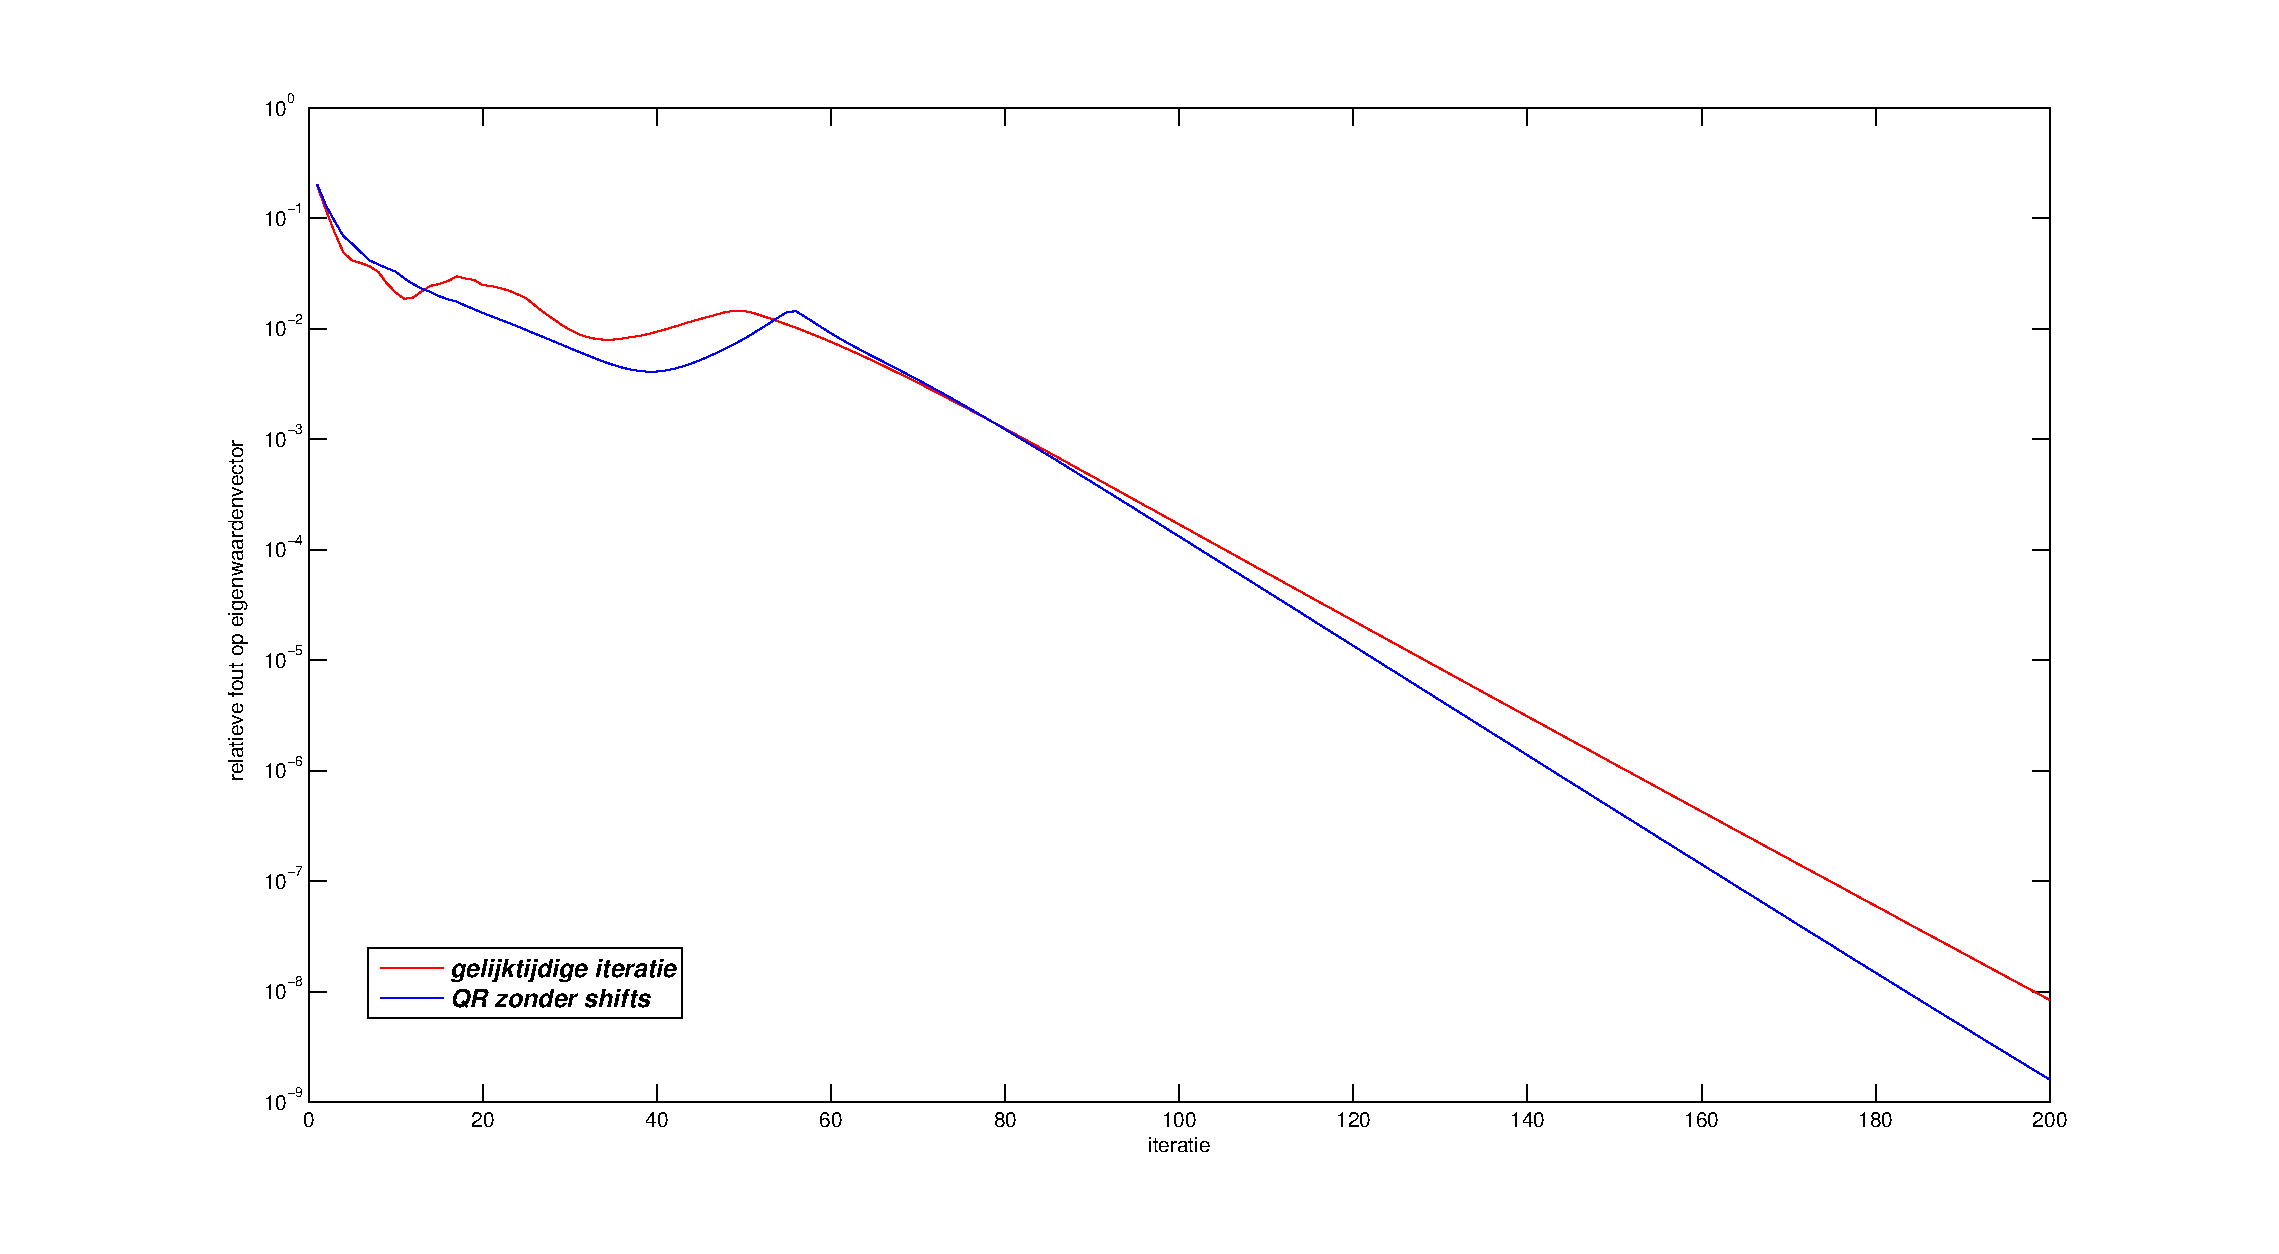
\includegraphics[width=0.8\textwidth]{vergelijkingLineair.eps}
	\caption{Vergelijking convergentie van unshifted QR en gelijktijdig iteratie}
	\label{vglSimQR}
\end{figure}

\subsection{Opgave 7}
We hebben een random ijle matrix $A \in \mathbb{R}^{1000\times1000}$ gegenereerd. Als we hierop de Arnoldi iteratie toepassen en de Ritz waarden berekenen voor elke iteratiestap krijgen we figuur \ref{arnoldiGraph}. We zien duidelijk dat er zeer snelle, geometrische convergentie is naar de extreme eigenwaarde 24.3868 die we berekend hebben met het commando $eigs(A)$. De andere eigenwaarden convergeren niet zo snel. 
\begin{figure}[htb]
	\begin{center}
	 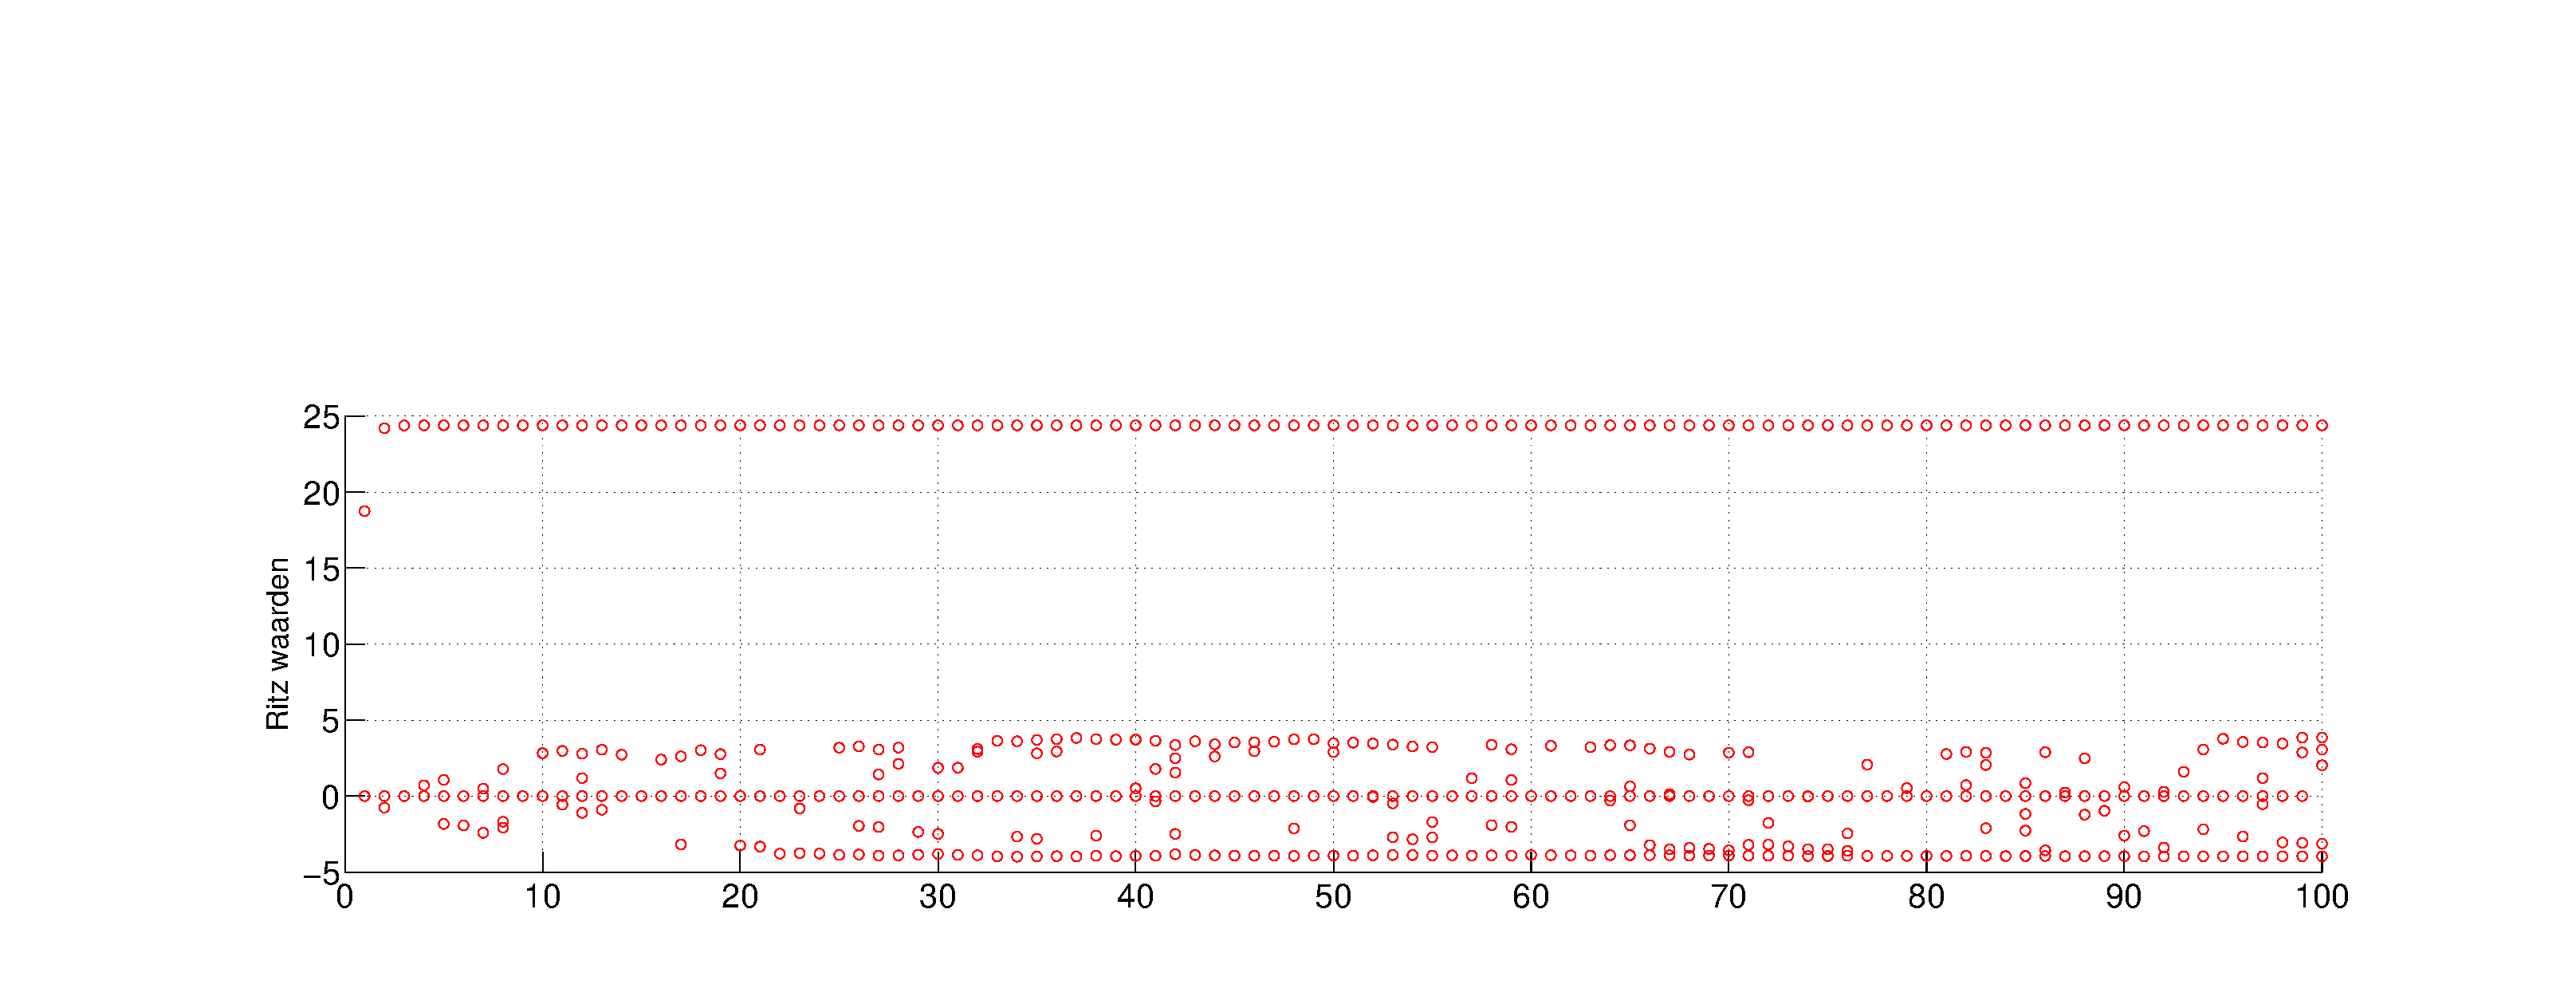
\includegraphics[width=\textwidth]{arnoldi.eps}
	\caption{Convergentie van Arnoldi-Ritz waarden}
	\label{arnoldiGraph}
	\end{center}

	
\end{figure}
\section{Alternatieve eigenwaardenalgoritmen}

\subsection{Opgave 8}
De Jacobi methode voor het vinden van eigenwaarden van een symmetrische matrix $A$ steunt op de vermenigvuldiging
\begin{equation} \label{jacobi}
 J^T\begin{bmatrix}a & d \\ d & b\end{bmatrix}J
\end{equation}
waarin geldt
\begin{equation} \label{Jacobimatrix}
 J=\begin{bmatrix}c & s\\ $-s$ & c\end{bmatrix}
\end{equation}
Hieronder zullen we de waarde van $s$ en $c$ berekenen zodat de niet-diagonaalelementen na de vermenigvuldiging \eqref{jacobi} gelijk zijn aan 0. \\
Aangezien het gaat om een rotatiematrix, moet de determinant van $J$ gelijk zijn aan 1.
\begin{equation}
 c^2+s^2=1
\end{equation}
Daarom kozen we voor volgende waarden voor $s$ en $c$
\begin{equation}
\begin{align}
 \begin{cases}
  c=\cos(\theta)\\
  s=\sin(\theta)
 \end{cases}
 \end{align}
\end{equation}
Dit geeft ons volgende uitdrukking voor de waarde van de niet-diagonaalelementen
\begin{equation} 
 \frac{1}{2}\sin(2\theta)(a-b) + d\cos(2\theta) = 0
\end{equation}
Verder uitwerken geeft ons
\begin{equation} \label{berekeningtheta}
 \theta = \frac{1}{2}\arctan(\frac{2d}{b-a})
\end{equation}
Als $a=b$ stellen we $\theta$ gelijk aan $\frac{\pi}{4}$, omdat bij die hoek de boogtangens oneindig is. 





\subsection{Opgave 9}
Tijdens een Jacobi iteratie zal de diagonaal van de matrix A overlopen worden, tot aan het voorlaatste diagonaalelement. Per diagonaalelement zal er in de rij gezocht worden naar het in absolute waarde grootste element verschillend van het diagonaalelement. Dit element zal geselecteerd worden omdat het de grootste impact heeft op het niet diagonaal zijn van de matrix. Daarom gaan we dit element verkleinen. Om dit te doen kiezen we als tweede diagonaalelement het element in dezelfde kolom als het grootste element. Met behulp van deze drie waarden en formule \eqref{berekeningtheta} berekenen we $\theta$. De J-matrix verkrijgen we door op een eenheidsmatrix met dezelfde dimensies als A  de overeenstemmende diagonaalelementen te vervangen door $\cos(\theta)$ en het element op de plaats van het grootste element en het spiegelbeeld van dit element te vervangen door respectievelijk $\sin(\theta)$ en $-\sin(\theta)$. Vervolgens vermenigvuldigt men matrix A langs links met $J^T$ om de rijen aan te passen en langs rechts met $J$ om de kolommen aan te passen.\\
Om een matrix met de bijhorende eigenvectoren te verkrijgen begint men met matrix V te initialiseren als een eenheidsmatrix. Bij elke vermenigvuldiging van $A$ met $J$ moet men V langs rechts vermenigvuldigen met J.\\
%vanuit de eenheidsmatrix door $I_{n,n}$ en $I_{m,m}$ te vervangen door $\cos(\theta)$ en $I_{m,n}$ door $-sin(\theta)$ en $I_{n,m}$ door $\sin(\theta)$

\begin{algorithmic}
 \STATE input(A,tol)  A = symmetrische matrix, tol = bovengrens voor de fout op een eigenwaarde 
 \STATE n = size(A)
 \STATE V = identitymatrix(n)
 \WHILE{maximum error \textgreater tol}
 	\FOR{ elk diagonaalelement behalve het laatste}
 \STATE 		max = kies het in grootste niet diagonaalelement van deze rij
 \STATE rij van diagonaalelement = n, m = kolom van max
 \STATE definieer a, b en d met $a=A_{n,n} b = A_{m,m}$ en $d = A_{n,m}$
 \STATE bepaal $\theta$ m.b.v \eqref{berekeningtheta}
 \STATE construeer Jacobimatrix J 
 \STATE $A = J^TAJ$
 \STATE $V = VJ $
	\ENDFOR
\ENDWHILE
\end{algorithmic}


\subsection{Opgave 10}
Als we onze implementatie van de Jacobi methode uitvoeren met matrix $mat1.txt$ als input en machineprecisie als tolerantie, krijgen we figuur \ref{jacobigraph}. We zien duidelijk dat de convergentie sneller dan lineair is, en eerder kwadratisch lijkt. Dit komt overeen met de theorie. \\
\begin{figure}[htb]
	\begin{center}
	 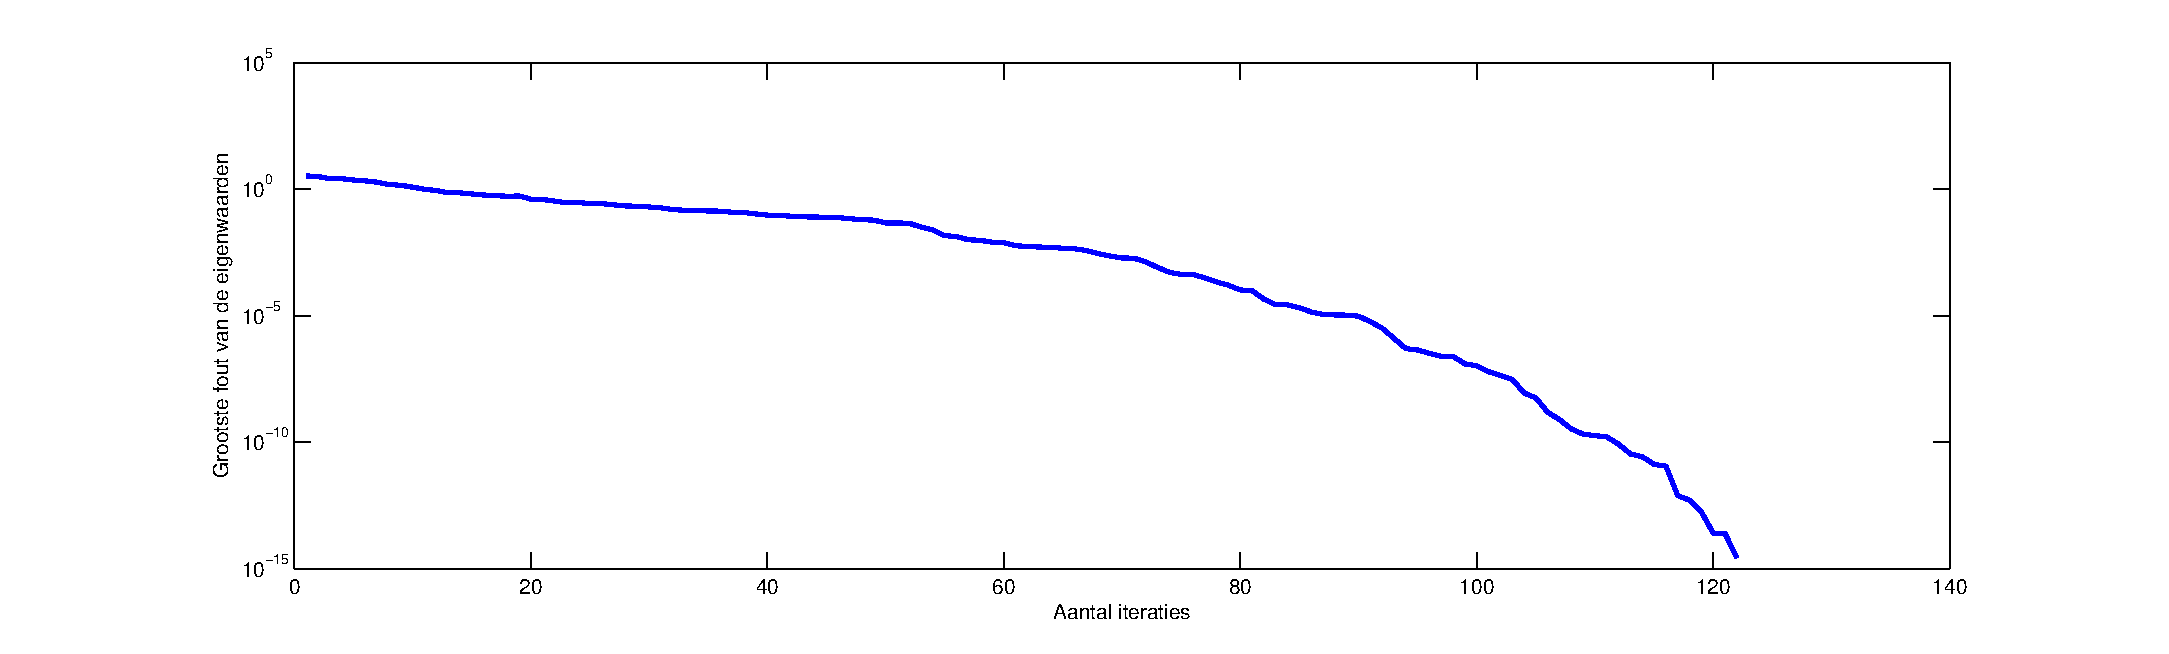
\includegraphics[width=\textwidth]{jacobi.eps}
	\caption{Convergentie van Jacobi methode}
	\label{jacobigraph}
	\end{center}
\end{figure}

Voor een symmetrische tridiagonale matrix $A \in \mathbb{R}^{m\times m}$ zijn er slechts $\mathcal{O}(m)$ elementen die gelijk moeten worden aan 0. Voor elke van deze elementen moet $\theta$ worden berekend en moeten er 3 matrixvermenigvuldigingen worden uitgevoerd. Na elke stap daalt de som van de kwadraten van de niet-diagonaalelementen met een constante factor. De convergentie kan dus gegarandeert worden na $\mathcal{O}(m^2\log(\epsilon_{mach}))$ stappen. Bij een volle matrix zouden er $\mathcal{O}(m^2)$ niet-nul elementen, en zouden er $m$ keer meer bewerkingen nodig zijn.\\
\section{Implementatie van de Jacobimethode}
\lstinputlisting[language=Matlab]{jacobitol.m}

\end{document}
